% AgriGraph AI — technical documentation (STGNN, backend, frontend).
% Target: ~15--20 pages at 11pt; compile with: pdflatex (twice) agrigraph_technologies_stgnn.tex
\documentclass[11pt,a4paper]{article}
\usepackage[utf8]{inputenc}
\usepackage[T1]{fontenc}
\usepackage{lmodern}
\usepackage{microtype}
\usepackage[margin=2.1cm]{geometry}
\usepackage{amsmath,amssymb}
\usepackage{booktabs}
\usepackage{tabularx}
\usepackage{enumitem}
\usepackage{hyperref}
\usepackage{bookmark}
\usepackage{multicol}
\usepackage{setspace}
\setstretch{1.35}
\usepackage{float}
\usepackage{tikz}
\usetikzlibrary{positioning,arrows.meta}

\hypersetup{colorlinks=true, linkcolor=blue!60!black, urlcolor=blue!60!black, pdftitle={AgriGraph AI Technical Documentation}}
\setlist{nosep,leftmargin=*}
\setlength{\emergencystretch}{2em}

\title{AgriGraph AI\\[0.4em]\large Technical Documentation\\[0.2em]\normalsize STGNN Pipeline, Backend API, and Frontend}
\author{}
\date{\small Generated from repository source layout. Version 0.1.0.}

\begin{document}
\maketitle

\begin{abstract}
\noindent
This document describes the AgriGraph AI prototype: the spatio-temporal graph neural network (STGNN) used for county-level sustainability scores, the Python/FastAPI backend (REST API, data flow, and training artifacts), and the React/Vite frontend (tabs, main user flows, and configuration). It is intended for developers and technical readers.
\end{abstract}

\tableofcontents
\clearpage

%----------------------------------------------------------------------
\section{Scope and data context}
%----------------------------------------------------------------------
The application ingests county-year dairy sustainability indicators (ICBF-style features), builds augmented training views, derives four PCA-based \emph{pillars} and an overall score, constructs a fixed spatial graph over the \textbf{26 Irish counties}, and trains an STGNN to forecast scores and support uncertainty and counterfactual tooling exposed via a REST API and consumed by a single-page web client.

Throughout this document, \textbf{Phase Ax} labels refer to the sequential pipeline modules under \texttt{backend/pipeline/} orchestrated by \texttt{run\_pipeline()}.

\begin{table}[H]
  \centering
  \caption{Pipeline modules invoked by \texttt{run\_pipeline()} (import names).}
  \label{tab:modules}
  \footnotesize
  \begin{tabular}{@{}ll@{}}
    \toprule
    \textbf{Phase} & \textbf{Python module (under \path{backend/pipeline/})} \\
    \midrule
    A1 & \path{data_loader.py} \\
    A2 & \path{preprocessing.py} \\
    A3 & \path{vae.py} \\
    A4--A5 & \path{pca_pillars.py} \\
    A6 & \path{graph.py} \\
    A7--A7b & \path{stgnn.py} \\
    A8 & \path{forecast.py} \\
    A9 & \path{uncertainty.py} \\
    A10 & \path{counterfactual.py} \\
    \bottomrule
  \end{tabular}
\end{table}

%----------------------------------------------------------------------
\section{End-to-end pipeline overview}
%----------------------------------------------------------------------
\subsection{Phase sequence}
Table~\ref{tab:phases} lists the research phases in execution order. The STGNN (\textbf{A7} evaluation training + metrics, \textbf{A7b} full-data retrain for forecasting) sits after graph construction and before downstream forecast export.

\begin{table}[H]
  \centering
  \caption{Pipeline phases (high level).}
  \label{tab:phases}
  \begin{tabular}{@{}ll@{}}
    \toprule
    \textbf{Phase} & \textbf{Role} \\
    \midrule
    A1 & Load and validate raw panel data \\
    A2 & Preprocessing / cleaning to standardized tables \\
    A3 & Year-conditioned CVAE training and feature augmentation (variants) \\
    A4/A5 & PCA pillars and sustainability scoring \\
    A6 & Spatial $k$-NN graph over counties (edge index for PyTorch Geometric) \\
    A7 / A7b & STGNN: honest metrics then forecast weights \\
    A8 & Forecast horizons and exports \\
    A9 & Uncertainty bands \\
    A10 & Counterfactual scenarios \\
    \bottomrule
  \end{tabular}
\end{table}

\subsection{Conceptual flow diagram}
Figure~\ref{fig:pipeline} summarises how preprocessing, augmentation, pillars, and the spatial graph feed the STGNN and downstream analytics.

\begin{figure}[H]
  \centering
  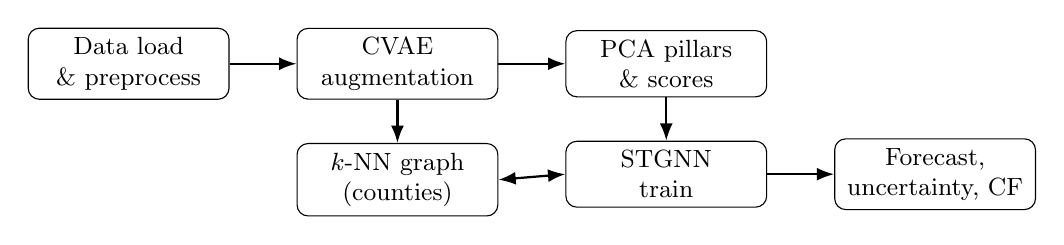
\begin{tikzpicture}[
    node distance=0.55cm and 0.85cm,
    box/.style={rectangle, draw, rounded corners, minimum width=2.55cm, minimum height=0.72cm, align=center, font=\small},
    arrow/.style={-{Latex[length=2.2mm]}, thick},
    darrow/.style={{Latex[length=2.2mm]}-{Latex[length=2.2mm]}, thick}
  ]
    \node[box] (a1) {Data load\\\& preprocess};
    \node[box, right=of a1] (a3) {CVAE\\augmentation};
    \node[box, right=of a3] (a4) {PCA pillars\\\& scores};
    \node[box, below=of a3] (a6) {$k$-NN graph\\(counties)};
    \node[box, below=of a4] (a7) {STGNN\\train};
    \node[box, right=of a7] (a8) {Forecast,\\uncertainty, CF};
    \draw[arrow] (a1) -- (a3);
    \draw[arrow] (a3) -- (a4);
    \draw[arrow] (a3.south) -- (a6.north);
    \draw[arrow] (a4.south) -- (a7.north);
    \draw[darrow] (a6.east) -- (a7.west);
    \draw[arrow] (a7) -- (a8);
  \end{tikzpicture}
  \caption{Abbreviated research pipeline: pillar scores and the county graph interact with STGNN training; subsequent phases consume the forecast-oriented model.}
  \label{fig:pipeline}
\end{figure}

%----------------------------------------------------------------------
\section{Spatial graph (Phase A6)}
%----------------------------------------------------------------------
\subsection{Construction}
Counties are nodes ($N=26$). Pairwise great-circle distances use the haversine formula on fixed centroid coordinates. A \textbf{$k$-nearest neighbour} adjacency is built per node (\texttt{K\_NEIGHBORS}${}=3$), then \textbf{symmetrised}: an undirected edge exists if either endpoint lists the other among its $k$ neighbours. Self-loops are removed.

\subsection{Artifacts}
Binary adjacency and a symmetric normalized Laplacian-style matrix are saved under \path{backend/artifacts/}; \path{edge_index.pt} stores directed edges for every undirected link (both directions) for PyTorch Geometric. County order is persisted in \path{graph_counties.pkl} and must stay aligned with STGNN node indexing.

%----------------------------------------------------------------------
\section{STGNN pipeline (Phases A7 and A7b)}
%----------------------------------------------------------------------
\subsection{Libraries}
Training and inference rely on:
\begin{itemize}
  \item \textbf{PyTorch} (\texttt{torch}) --- modules, Adam optimiser, automatic differentiation;
  \item \textbf{PyTorch Geometric} --- \texttt{GCNConv} for graph convolution;
  \item \textbf{NumPy / pandas} --- tabular IO and metric computation;
  \item \textbf{scikit-learn} --- $R^2$, MAE, MSE on held-out predictions.
\end{itemize}

\subsection{Node features and temporal tensor}
For each variant ID and each input year in \texttt{INPUT\_YEARS}${}=[2021,2022,2023,2024]$, the model builds a snapshot tensor of shape $(N, F)$ with $F=5$:
\begin{itemize}
  \item Four pillar dimensions (from augmented pillar scores);
  \item One \textbf{lag-normalised} prior-year score channel (computed from sustainability scores with global lag statistics \texttt{y\_bar}, \texttt{sigma\_y}).
\end{itemize}
The full input to the network is therefore $X \in \mathbb{R}^{T \times N \times F}$ with $T=4$, $N=26$, $F=5$.

\subsection{Targets and scaling}
The regression target is the county sustainability \textbf{score for year 2025} (per variant). Targets are \textbf{standardised} using the mean and standard deviation of scores computed from the training frames (saved as \texttt{stgnn\_target\_scaler.pkl}). Predictions are inverted to the original score scale for evaluation and reporting.

\subsection{Architecture}
The class \texttt{STGNN} (\texttt{backend/pipeline/stgnn.py}) implements:
\begin{enumerate}
  \item \textbf{Spatial stack (per timestep)}: two \texttt{GCNConv} layers: $F_{\mathrm{in}}{=}5 \rightarrow 64 \rightarrow 64$, each followed by ReLU and dropout ($p{=}0.2$).
  \item \textbf{Temporal pooling}: for each timestep $t$, node embeddings $h_t \in \mathbb{R}^{N \times 64}$ are projected to queries, keys, and values in dimension $d{=}32$. Attention uses the \textbf{last} timestep's query against all timesteps' keys; a \textbf{causal} mask zeros out contributions from future timesteps so the final step cannot attend upward in time within the window.
  \item \textbf{Head}: linear $32\rightarrow32$, ReLU, then $32\rightarrow16\rightarrow1$ producing one scalar per county (shape $(N,)$).
\end{enumerate}

\subsection{Training logs}
Intermediate diagnostics print at epochs \texttt{LOG\_EPOCHS}${}=(1,100,250,500)$ and always at the final epoch (500). Logs report phase tags such as \texttt{A7-fold1}..\texttt{A7-fold4}, \texttt{A7-final}, and \texttt{A7b}.

\subsection{Hyperparameters and optimisation}
Table~\ref{tab:stgnn-hparams} lists the main constants in code.

\begin{table}[H]
  \centering
  \caption{STGNN training hyperparameters (from \texttt{CONSTANTS} in \texttt{stgnn.py}).}
  \label{tab:stgnn-hparams}
  \begin{tabular}{@{}ll@{}}
    \toprule
    \textbf{Symbol / key} & \textbf{Value} \\
    \midrule
    \texttt{GCN\_HIDDEN} & 64 \\
    \texttt{ATTN\_DIM} & 32 \\
    \texttt{HEAD\_HIDDEN} & 16 \\
    \texttt{DROPOUT} & 0.2 \\
    \texttt{EPOCHS} & 500 \\
    \texttt{LEARNING\_RATE} & $10^{-3}$ \\
    \texttt{WEIGHT\_DECAY} & $10^{-4}$ \\
    \texttt{SEED} & 42 \\
    \texttt{INPUT\_YEARS} & 2021--2024 (4 timesteps) \\
    \texttt{TARGET\_YEAR} & 2025 \\
    \texttt{REAL\_VARIANT\_ID} & 0 (non-augmented) \\
    \texttt{SYNTHETIC\_VARIANTS} & $\{1,2,3,4\}$ \\
    \bottomrule
  \end{tabular}
\end{table}

The optimiser is \textbf{Adam} with parameters above. The training loss is \textbf{mean squared error} averaged over all training variants used in the step: for each variant~$v$, the model predicts $\hat{y}_v \in \mathbb{R}^N$ and minimises $\lVert \hat{y}_v - y_v \rVert^2$ aggregated across variants and nodes (exact averaging matches the implementation in \texttt{\_train\_one\_run}).

\subsection{Phase A7 --- evaluation protocol}
\begin{itemize}
  \item \textbf{$k$-fold on synthetic variants}: each of the four synthetic variant IDs is held out once as validation while the other three train (same epoch budget each fold). Training and validation $R^2$ are computed \textbf{on scaled targets}, pooled over nodes and variants in the split.
  \item \textbf{Final eval model}: train on \emph{all} synthetic variants $\{1,2,3,4\}$, then evaluate on the \textbf{real} variant ($0$) for year~2025 only --- metrics reported as test $R^2$, MAE, MSE (and normalised MAE/MSE). This is the honest generalisation signal for the UI metrics endpoint.
  \item \textbf{Outputs:}\\
        {\small \path{models/stgnn_eval_weights.pt}, \path{artifacts/stgnn_metrics.json}, \path{artifacts/stgnn_eval_predictions.csv}.}
\end{itemize}

\subsection{Phase A7b --- forecast weights}
A second model is trained on \textbf{all} variants $\{0,1,2,3,4\}$ with the same architecture and epochs. \textbf{No additional test metrics} are computed for this run; its weights drive operational forecasting and downstream phases. Output: \texttt{models/stgnn\_forecast\_weights.pt}.

\textbf{Important:} Do not report A7b training as ``test performance'' --- there is no held-out year for that fit.

\subsection{Key artifact filenames}
\begin{center}
\footnotesize
\begin{tabular}{@{}l p{8.2cm}@{}}
  \toprule
  \textbf{File} & \textbf{Purpose} \\
  \midrule
  \path{edge_index.pt} & PyG edge list for GCN \\
  \path{stgnn_forecast_weights.pt} & Deployed STGNN state dict + metadata \\
  \path{stgnn_eval_weights.pt} & Eval-focused weights for metrics lineage \\
  \path{stgnn_metrics.json} & A7 fold and test metrics \\
  \path{stgnn_target_scaler.pkl} & Target mean/std for (de)normalisation \\
  \path{lag_norm.pkl} & Lag-channel normalisation stats \\
  \bottomrule
\end{tabular}
\end{center}

%----------------------------------------------------------------------
\section{Upstream modelling (CVAE and PCA pillars)}
%----------------------------------------------------------------------
\subsection{Conditional VAE augmentation (Phase A3)}
The CVAE expands each real county-year row into additional synthetic \emph{variant} rows (\texttt{variant\_id}${}\in\{1,2,3,4\}$) while preserving year conditioning. Training uses PyTorch \texttt{nn} modules, Adam optimiser, batch size~32, $\beta{=}1$, latent dimension~80, hidden width~128, and 200~epochs with fixed seed~42. Synthetic diversity is checked against quality thresholds on mean absolute feature drift and correlation-matrix distance (\texttt{MEAN\_ABS\_DIFF\_THRESHOLD}${}=0.05$, \texttt{CORRELATION\_NORM\_THRESHOLD}${}=7.0$). Primary artefacts: \path{backend/models/cvae_weights.pt}, \path{backend/data/x_augmented.csv}, and JSON logs under \path{backend/artifacts/}.

\begin{table}[H]
  \centering
  \caption{Selected CVAE configuration keys (\texttt{vae.py}).}
  \label{tab:cvae}
  \begin{tabular}{@{}ll@{}}
    \toprule
    \textbf{Key} & \textbf{Value} \\
    \midrule
    \texttt{INPUT\_DIM} & 17 herd features \\
    \texttt{CONDITION\_DIM} & 5 (year one-hot + metadata) \\
    \texttt{LATENT\_DIM} & 80 \\
    \texttt{HIDDEN\_DIM} & 128 \\
    \texttt{EPOCHS} & 200 \\
    \texttt{LEARNING\_RATE} & $10^{-3}$ \\
    \texttt{BATCH\_SIZE} & 32 \\
    \texttt{SYNTHETIC\_PER\_REAL} & 4 \\
    \bottomrule
  \end{tabular}
\end{table}

\subsection{PCA pillars and scores (Phases A4--A5)}
Seventeen standardised features feed PCA; \textbf{four} components are retained as pillars (\texttt{N\_COMPONENTS\_RETAINED} equals four). Pillar interpretation uses loadings with a \textbf{75th-percentile} dominant-feature rule; some features are marked negative-polarity so that ``higher is better'' aligns across indicators. Scores are mapped to $[0,100]$ for presentation. Frozen transforms (\path{standard_scaler.pkl}, \path{pca_loadings.npy}, \path{pillar_weights.pkl}, \path{score_params.pkl}) are consumed at API time for live pillar preview and counterfactual paths. The full feature set is listed in Appendix~\ref{app:features}.

%----------------------------------------------------------------------
\section{Downstream of the STGNN: forecast, uncertainty, counterfactuals}
%----------------------------------------------------------------------
\subsection{Autoregressive forecast (Phase A8)}
Phase~A8 reloads the \textbf{forecast} STGNN checkpoint (\path{stgnn_forecast_weights.pt}) and rolls the model forward year by year from~2026 to~2036. It builds each year's input window from historical and extrapolated pillar trajectories, applying percentile-based guards on pillars, lags, and score dynamics, and optional out-of-distribution (OOD) blending so extreme extrapolations are damped. Rolling windows use \texttt{WINDOW\_INPUT\_YEARS}${}=[2022,2023,2024,2025]$ as the four-step input after the first forecast year. OOD detection combines normalised pillar, lag, and score signals with weights $0.45/0.25/0.30$; blend factors \texttt{BLEND\_WEIGHT\_LOW/MEDIUM/HIGH} default to $0.85/0.55/0.25$ for low/medium/high OOD scores. Outputs: \path{forecast_2026_2036.csv} and \path{forecast_pillars_2026_2036.csv}.

\subsection{Monte Carlo uncertainty (Phase A9)}
Uncertainty bands are generated by adding Gaussian noise in \textbf{score space} to the A8 forecast and taking empirical 5th/95th percentiles per county-year. Key parameters: \texttt{MONTE\_CARLO\_TRIALS}${}=100$, \texttt{SIGMA\_MC}${}=0.1$, random seed~42, with scores clipped to $[0,100]$ after perturbation. Output: \path{uncertainty_bands.csv}, merged by the \path{/forecast} API.

\subsection{Counterfactual simulation (Phase A10)}
The counterfactual engine (\texttt{counterfactual.py}) composes user intervention vectors with the same frozen transforms and STGNN-based dynamics used in training, returning baseline and scenario score paths, per-pillar shifts, and short natural-language explanations (\texttt{backend/api/explanation.py}). Endpoints: \path{/counterfactual} and \path{/counterfactual/global}.

%----------------------------------------------------------------------
\section{Backend: technologies and behaviour}
%----------------------------------------------------------------------
\subsection{Stack and dependencies}
Table~\ref{tab:pydeps} lists pinned Python packages from \texttt{backend/requirements.txt}.

\begin{table}[H]
  \centering
  \caption{Backend Python dependencies (versions as in repository).}
  \label{tab:pydeps}
  \begin{tabular}{@{}ll@{}}
    \toprule
    \textbf{Package} & \textbf{Role} \\
    \midrule
    FastAPI & HTTP API framework, routing, request validation \\
    Uvicorn & ASGI server \\
    pandas / NumPy / SciPy & Data frames, numerics \\
    scikit-learn & PCA, scaling, metrics \\
    PyTorch & Deep learning (CVAE, STGNN) \\
    torch-geometric & Graph convolution layers \\
    python-multipart & Form/file uploads if needed \\
    \bottomrule
  \end{tabular}
\end{table}

\subsection{Application entrypoint}
\texttt{backend/main.py} constructs a FastAPI app with:
\begin{itemize}
  \item \textbf{Lifespan startup}: if \texttt{stgnn\_forecast\_weights.pt} or \texttt{data/forecast\_2026\_2036.csv} is missing, it runs the \textbf{full offline pipeline} (\texttt{run\_pipeline()}). Otherwise it skips training and only loads cached state.
  \item \textbf{CORS}: allows origin \texttt{http://localhost:5173} (Vite dev server).
  \item \textbf{Cache headers}: \texttt{Cache-Control: no-store} on \texttt{/api} responses to avoid stale JSON after regenerating artifacts.
  \item \textbf{Routes}: API router mounted at prefix \texttt{/api}; health check at \texttt{/health}.
\end{itemize}

\subsection{Loaded application state}
\texttt{load\_state()} (\texttt{backend/api/state.py}) builds an \texttt{AppState} containing: frozen PCA/pillar transforms, county list, historical and forecast score tables, uncertainty bands, augmented and forecast pillar panels, normalised feature table for slider previews, STGNN metrics JSON, and human-readable pillar label keys for API responses.

\subsection{REST API summary}
\noindent
Table~\ref{tab:api} lists the main HTTP endpoints. All paths below are relative to the API base \texttt{/api}; the health route is an exception.

{\footnotesize
\begin{table}[H]
  \centering
  \caption{REST API endpoints exposed by the FastAPI application.}
  \label{tab:api}
  \begin{tabularx}{\linewidth}{@{}l l X@{}}
    \toprule
    \textbf{Path} & \textbf{Method} & \textbf{Description} \\
    \midrule
    \path{/health} & GET & Liveness (\texttt{\{"status":"ok"\}}); mounted at app root, not under \texttt{/api}. \\
    \path{/counties} & GET & Sorted list of valid county names. \\
    \path{/historical} & GET & Historical county-year scores. \\
    \path{/forecast} & GET & Forecast scores merged with 5th/95th uncertainty bands. \\
    \path{/pillars/{county}} & GET & Pillar time series (historical + forecast) with normalised display columns. \\
    \path{/pillars/preview} & POST & Instant pillar change from intervention deltas (frozen PCA transform). \\
    \path{/counterfactual} & POST & County simulation: baseline vs scenario trajectories, pillar shifts, explanation text. \\
    \path{/counterfactual/global} & POST & Multi-county scenarios for coordinated simulation. \\
    \path{/comparison} & GET & STGNN vs linear-trend vs county-mean baselines. \\
    \path{/metrics} & GET & Aggregated A7 test and fold metrics. \\
    \path{/county/{county}/indicators} & GET & Score plus selected raw indicators (optional query \texttt{year}). \\
    \path{/methodology/learning_curves} & GET & CVAE history JSON + STGNN fold $R^2$ pairs. \\
    \path{/methodology/cvae_validation} & GET & Real vs synthetic summary stats for methodology UI. \\
    \bottomrule
  \end{tabularx}
\end{table}
}

\subsection{Request bounds (illustrative)}
Pillar preview applies bounded multiplicative deltas to normalised feature vectors (\texttt{DELTA\_MIN}${}=-1$, \texttt{DELTA\_MAX}${}=1$), then clips to $[0,1]$ before the frozen pillar transform. Counterfactual requests accept a \texttt{horizon} (default long horizon in single-county; global default often 11 years in line with UI).

\subsection{Forecast baselines (\texttt{/comparison})}
The endpoint \path{/comparison} returns three trajectories per county-year for 2026--2036: \textbf{STGNN} forecasts from cached CSVs, a \textbf{linear trend} baseline (per-county linear regression over 2021--2025 extended forward), and a \textbf{county mean} baseline that repeats each county's 2025 score flat across the horizon. These baselines are for comparative analytics only and do not replace the operational STGNN forecast path.

%----------------------------------------------------------------------
\section{Frontend: technologies and usage}
%----------------------------------------------------------------------
\subsection{Stack}
\begin{itemize}
  \item \textbf{React 18} with \textbf{Vite} as the dev server and bundler;
  \item \textbf{Tailwind CSS} for utility-first styling (including dark mode toggle on the root document);
  \item \textbf{Recharts} for time series, bands, and radar charts;
  \item \textbf{react-simple-maps} + \textbf{topojson-client} for the Ireland county map;
  \item \textbf{React Router} is a dependency (routing usage is minimal in the scaffold but available for expansion).
\end{itemize}

\subsection{API configuration}
The client expects the backend at \texttt{http://localhost:8000}. All JSON requests use the base URL defined in \texttt{frontend/src/config.js}:
\begin{verbatim}
export const API_BASE_URL = "http://localhost:8000/api";
\end{verbatim}
Change this if you proxy through another host or deploy behind TLS.

\subsection{Main UI structure}
The shell in \texttt{App.jsx} defines three tabs: \textbf{Atlas}, \textbf{Benchmarks}, \textbf{Methodology}. Shared props include the county list, selected county/year, historical and forecast rows fetched at startup, and (for Atlas/Benchmarks) global counterfactual simulation state.

\subsubsection{Atlas}
Primary exploratory view: map-based county selection, sustainability trajectory with forecast band, pillar radar and per-pillar charts, simulation sidebar (scenarios, sliders, pillar preview), and optional counterfactual result layout after running the global simulation.

\subsubsection{Benchmarks}
County ranking and comparison views using merged timelines and KPI-style summaries; can link behaviour back to Atlas via props (e.g.\ confirming county focus).

\subsubsection{Methodology}
Static and data-driven explanation of the pipeline: learning curves and CVAE validation fetched from \texttt{/methodology/*} endpoints.

\subsection{Typical local workflow}
\begin{enumerate}
  \item Install backend dependencies once: \texttt{pip install -r backend/requirements.txt} inside your Python environment.
  \item Start API from repository root: \texttt{uvicorn backend.main:app}. Use \texttt{--reload} only when editing Python sources (it watches files and restarts the server).
  \item Install frontend packages once: \texttt{cd frontend \&\& npm install}.
  \item Start Vite: \texttt{npm run dev}; open \texttt{http://localhost:5173}.
  \item Verify \texttt{GET http://localhost:8000/health}. If \path{stgnn_forecast_weights.pt} or \path{forecast_2026_2036.csv} is missing, startup triggers \texttt{run\_pipeline()} and may run for a long time on first boot.
\end{enumerate}

\subsection{Atlas tab (primary workflow)}
\begin{enumerate}
  \item Wait for counties and base timelines to load (spinner clears).
  \item Select a county on the map or list; optionally adjust the analysis year on any chart control that exposes it.
  \item Inspect sustainability trajectory (historical vs forecast with uncertainty ribbon where applicable) and pillar radar / per-pillar trends.
  \item Open the simulation sidebar: pick scenario chips or edit sliders representing herd interventions.
  \item Use pillar preview (POST \path{/pillars/preview}) for immediate feedback; run the global counterfactual when ready --- the app batches scenarios and POSTs to \path{/counterfactual/global}.
  \item Switch simulation result toggles to compare baseline vs intervention layouts when results return.
\end{enumerate}

\subsection{Benchmarks tab}
Use this tab for cross-county comparison views and KPI rankings fed by the same cached forecast/historical payloads; simulation hooks may delegate focus back to Atlas depending on UI state.

\subsection{Methodology tab}
Static narrative plus charts sourced from \path{/methodology/learning_curves} (CVAE loss history and STGNN fold $R^2$ bars) and \path{/methodology/cvae_validation} (real vs synthetic moments).

\subsection{Frontend module map (concise)}
\begin{center}
\small
\begin{tabular}{@{}lp{9cm}@{}}
  \toprule
  \textbf{Area} & \textbf{Role} \\
  \midrule
  \texttt{src/api.js} & Fetch wrappers, timeline helpers, score tiers \\
  \texttt{src/views/AtlasView.jsx} & Map + dashboard + simulation orchestration \\
  \texttt{src/views/BenchmarksView.jsx} & Rankings and comparative charts \\
  \texttt{src/views/MethodologyView.jsx} & Pipeline narrative and methodology charts \\
  \texttt{src/components/PillarRadar.jsx} & Four-pillar radar chart \\
  \texttt{src/components/atlas/*} & Map, sidebars, charts, simulation toggles \\
  \bottomrule
\end{tabular}
\end{center}

%----------------------------------------------------------------------
\section{Operational notes}
%----------------------------------------------------------------------
\begin{itemize}
  \item \textbf{Single source of truth for metrics}: use \path{/api/metrics} and \path{artifacts/stgnn_metrics.json} for A7 test numbers only.
  \item \textbf{Forecast weights}: production forecasting and uncertainty pipelines must consume \path{stgnn_forecast_weights.pt}, not the eval checkpoint.
  \item \textbf{Reproducibility}: STGNN training fixes NumPy and PyTorch RNG seeds to 42 (CPU training in code paths inspected).
\end{itemize}

\subsection{Pillar display scaling (API)}
Endpoints returning pillar rows attach normalised display columns by clipping each pillar $z$-score to $[-3,3]$ then linearly mapping to $[0,100]$ with unit spacing proportional to a six-point span (\texttt{routes.py}). These columns power radar charts; underlying PCA values remain in statistical units.

\subsection{CORS and deployment}
The API permits browser requests only from \texttt{http://localhost:5173}. Deploying the frontend elsewhere requires updating \texttt{FRONTEND\_ORIGIN} in \path{backend/main.py} and \texttt{API\_BASE\_URL} in \path{frontend/src/config.js} consistently. Reverse proxies should forward \path{/api} and disable caching for JSON (the middleware already sets no-store for \path{/api}).

\subsection{Illustrative JSON payloads}
\noindent\textbf{Pillar preview} (\texttt{POST /api/pillars/preview}): intervention keys must match engineered feature names (see Appendix~\ref{app:features}). Example body:
\begin{verbatim}
{
  "county": "Tipperary",
  "interventions": { "calving_interval": -0.02 }
}
\end{verbatim}
\noindent\textbf{Single-county counterfactual} (\texttt{POST /api/counterfactual}): includes optional long-range \texttt{horizon} (years simulated beyond baseline mechanics).

\noindent\textbf{Global counterfactual} (\texttt{POST /api/counterfactual/global}): expects \texttt{scenarios} as a map \texttt{\{ "<County>": \{ "<feature>": <delta>, ... \}, ... \}} plus \texttt{horizon} for simultaneous multi-county runs.

%----------------------------------------------------------------------
\appendix
\section{Tensor shapes and attention mask}
Let $T{=}4$, $N{=}26$, $F{=}5$. The module receives $X\in\mathbb{R}^{T\times N\times F}$ and \texttt{edge\_index} with shape $(2,E)$. After spatial GCN blocks, tensors $Q,K,V\in\mathbb{R}^{T\times N\times d}$ are formed with $d{=}32$. Attention logits for the final timestep use row $T{-}1$ of $Q$ against all rows of $K$; entries corresponding to future timesteps are masked to $-\infty$ before softmax, enforcing causality within the window.

\section{Repository locations (reference)}
\begin{center}
\footnotesize
\begin{tabular}{@{}lp{9cm}@{}}
  \toprule
  \textbf{Path} & \textbf{Contents} \\
  \midrule
  \path{backend/main.py} & FastAPI app, CORS, lifespan, router mount \\
  \path{backend/api/routes.py} & REST endpoints and request models \\
  \path{backend/api/baselines.py} & Linear trend and flat county baselines \\
  \path{backend/pipeline/} & Phases A1--A10 modules \\
  \path{backend/data/} & CSV inputs and generated panels \\
  \path{backend/models/} & CVAE and STGNN weight files \\
  \path{backend/artifacts/} & Metrics JSON, CVAE logs, graph matrices \\
  \path{frontend/src/} & React application source \\
  \bottomrule
\end{tabular}
\end{center}

\section{ICBF feature columns used in PCA}
\label{app:features}
The following 17 columns (see \texttt{pca\_pillars.py} \texttt{FEATURE\_COLS}) are standardised before PCA. Order is fixed in the pipeline.
\begin{multicols}{2}
\footnotesize
\begin{itemize}
  \item \texttt{num\_herds}
  \item \texttt{calving\_interval}
  \item \texttt{six\_wk\_calving\_rate}
  \item \texttt{calves\_per\_cow\_per\_year}
  \item \texttt{females\_not\_calved\_pct}
  \item \texttt{avg\_lactations}
  \item \texttt{current\_replacement\_rate}
  \item \texttt{potential\_replacement\_rate}
  \item \texttt{cows\_culled\_pct}
  \item \texttt{heifers\_calved\_22\_26mo}
  \item \texttt{mortality\_dead\_at\_birth}
  \item \texttt{mortality\_dead\_28days}
  \item \texttt{replacements\_dairy\_ai\_pct}
  \item \texttt{births\_known\_sire\_pct}
  \item \texttt{births\_calving\_survey\_pct}
  \item \texttt{recycled\_cows\_pct}
  \item \texttt{autumn\_6wk\_calving\_rate}
\end{itemize}
\end{multicols}

\section*{Glossary (selected)}
\begin{description}[style=sameline,leftmargin=3.2cm]
  \item[Variant ID] Index $0$ denotes observed (real) rows; $1$--$4$ denote CVAE-derived synthetic replicates for the same county-year stratum.
  \item[Pillar] One of four PCA-derived orthogonal summaries of herd indicators before interpretation labelling.
  \item[Lag channel] Fifth STGNN input feature carrying normalised prior-year score inertia per county.
  \item[Eval weights] STGNN checkpoint trained for held-out metrics on real 2025 scores (Phase A7 lineage).
  \item[Forecast weights] STGNN checkpoint trained on all variants for operational rollout (Phase A7b).
  \item[OOD blend] Mechanism in Phase A8 that reduces reliance on wild extrapolations when pillar/lag/score trajectories look inconsistent with historical envelopes.
\end{description}

\section*{Disclaimer}
This documentation mirrors the current codebase structure. Numerical results depend on input CSVs and trained weights under \path{backend/data/} and \path{backend/models/}. Regenerating artefacts changes forecasts and metrics.

\end{document}
